\section*{Modulebeschrijving}
\begin{tabularx}{\textwidth}{|>{\columncolor{lichtGrijs}} p{.26\textwidth}|X|}
	\hline
	\textbf{Module name:} & \modulenaam\\
	\hline
	\textbf{Module code: }& \modulecode\\
	\hline
	\textbf{Study points \newline and hours of effort:} & This module gives \stdPunten, in correspondance with 112 hours:
	\begin{itemize}
		\item 3 x 6 hours frontal lecture
		\item 3 x 6 hours practicum
		\item the rest is self-study
	\end{itemize} \\
	\hline
	\textbf{Examination:} & Written examination and practicums (with oral check) \\
	\hline
	\textbf{Course structure:} & Lectures, self-study, and practicums \\
	\hline
	\textbf{Prerequisite knowledge:} & None. \\
	\hline
	\textbf{Learning tools:}  &
		\begin{itemize}
			\item Book: Think Python; author A. B. Downey (\url{http://www.greenteapress.com/thinkpython/})
			\item Presentations (in pdf): found on N@tschool and on the GitHub repository \url{https://github.com/hogeschool/INFDEV01-1}
			\item Assignments, to be done at home and during practical lectures (pdf): found on N@tschool and on the GitHub repository \url{https://github.com/hogeschool/INFDEV01-1}
		\end{itemize} \\
	\hline
	\textbf{Connected to \newline competences:} &
	\begin{center}
		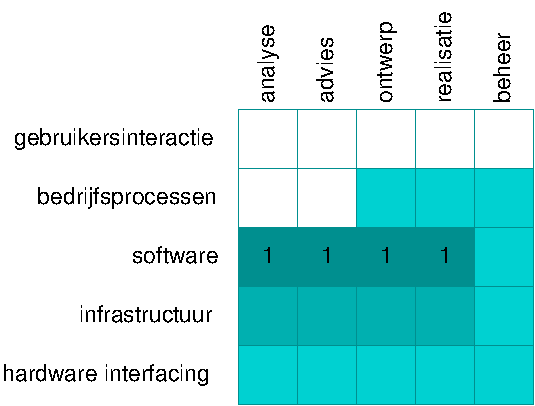
\includegraphics[width=7cm]{img/comptabel.pdf}
	\end{center}\\
	\hline
	\textbf{Learning objectives:} &
		At the end of the course, the student can:
			\begin{itemize}
				\item \textbf{understand and describe} the logical model of computation \texttt{LMC}
				\item \textbf{understand and describe} the concrete model of computation \texttt{CMC}
				\item \textbf{use} variables and basic data types \texttt{VAR}
				\item \textbf{use} arithmetic and boolean expressions \texttt{EXPR}
				\item \textbf{use} conditional control-flow statements \texttt{COND}
				\item \textbf{use} looping control-flow statements \texttt{LOOP}
			\end{itemize} \\
		
	\hline
\end{tabularx}
\newpage

\begin{tabularx}{\textwidth}{|>{\columncolor{lichtGrijs}} p{.26\textwidth}|X|}
	\hline
	\textbf{Content:}&
	\begin{itemize}
		\item basic concepts of computation from a logical standpoint
		\item basic concepts of computation from a concreter perspective in terms of storage and instructions
		\item variables (in Python 2)
		\item primitive datatypes and expressions (in Python 2)
		\item conditional control-flow statements (in Python 2)
		\item looping control-flow statements (in Python 2)
	\end{itemize} \\
	\hline
	\textbf{Course owners:} & \author\\
	\hline
	\textbf{Date:} & \today \\
	\hline
\end{tabularx}
\newpage
